% !TEX root = ../main.tex
\subsubsection{The Parton Model}
\label{10.12::parton_model}
    \begin{figure}[t!]
        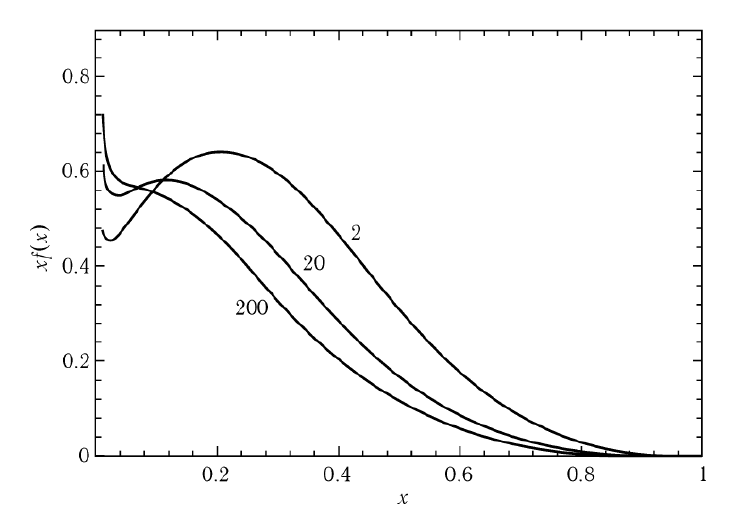
\includegraphics[width=0.8\textwidth]{12q2_dependence_u.png}
        \caption[$Q^2$ dependence of $x$ PDF for the $u$ quark.]
        {Parton distribution functions $xf_f(x)$ for the $u$ quark at $Q = 2$, $Q = 20$, and $Q = 200$ GeV, showing the parton evolution effect according to the Altarelli-Parisi equations.}
        % NOTE. Can't find a source :(.
        \label{fig::10.12::q2_dependence}
    \end{figure}

    In the parton model, the cross section is given by
    \begin{equation}
        \frac{d^2\sigma}{dxdy} \left( e^-p \rightarrow e^-X \right) =
            \left( \sum_f xf_f \left( x, Q^2 \right) Q_f^2 \right)
            \frac{2\pi\alpha s}{Q^4} \left( 1 + \left( 1 - y \right)^2 \right),
        \label{eq::10.12::parton_model_cross_section}
    \end{equation}
    where $s \equiv 2P\cdot k$, $Q_f$ represents the charge of parton $f$, and $x$ and $y$ are the Bjorken variables defined as
    \begin{equation*}
        x \equiv \frac{Q^2}{2P\cdot q}, \hspace{36pt} y \equiv \frac{2 P\cdot q}{s}.
    \end{equation*}
    In the nucleon's rest frame, $y = q^0/k^0$, and it represents the energy transferred to the hadron by the incoming electron.

    The PDFs in Equation \eqref{eq::10.12::parton_model_cross_section} have a weak dependence on $Q^2$ due to gluon radiation.
    This leads to Bjorken scaling violation \cite{halzen1991}.
    When the structure functions are known for certain values of $Q^2$, they can be evolved to other values using the Dokshitzer-Gribov-Lipatov-Altarelli-Parisi (DGLAP) equations \cite{dokshitzer1991}.

    Figure \ref{fig::10.12::q2_dependence} shows the predictions of the Altarelli-Parisi equations for the evolution of the PDFs with respect to $Q^2$.
    Partons with large $x$ tend to radiate and move towards states with lower $x$ values.
    Simultaneously, radiation generates new partons with low $x$ values.
    As $Q^2$ increases, the parton distributions decrease for large $x$ values while rapidly increasing for low $x$.
    At low $Q^2$, the wavelength of the virtual photon is too large to probe the partons directly, resulting in probing the proton as a whole.
    The precise range of validity for the QCD-extended parton model is not known, but it is assumed to be applicable for $Q^2 > 1 \text{ GeV}^2$, corresponding to a spatial resolution of approximately $0.2$ fm.
